\documentclass
% Uncomment to get one page per frame
%[handout]
{beamer}

\usepackage{amsfonts}
\usepackage{amsmath}
\usepackage{longtable}
\usepackage{csquotes}
\usepackage{standalone}

\usepackage{graphicx}
\graphicspath{{../pictures/}}

\usepackage{tikz}
\usetikzlibrary{shapes, calc, arrows, decorations.markings,
  decorations.pathmorphing, decorations, patterns, chains, snakes,
  backgrounds, positioning, fit, petri}
\newcommand{\inputpicture}[1]{\input{../drawings/#1}}

\newcommand{\reg}{\textsuperscript{\textregistered}}

\usepackage{listings}
\lstset{language=C, basicstyle=\ttfamily, breaklines=true, keepspaces=true,
  keywordstyle=\color{blue}}

\usepackage{bytefield}

\usefonttheme{professionalfonts}
\usefonttheme{serif}
\usepackage{fontspec}
\setromanfont{CMU Serif}
\setsansfont{CMU Sans Serif}
\setmonofont{CMU Typewriter Text}

\newcommand{\No}{{\fontfamily{lmr}\selectfont \textnumero}}

\usepackage{hyperref}
\hypersetup{colorlinks=true, linkcolor=black, filecolor=black, citecolor=black,
  urlcolor=blue , pdfauthor=Evgenii Iuliugin <yulyugin@gmail.com>,
  pdftitle=Fundamentals of Full-Platform Simulation}

\usepackage{underscore}
\usepackage{amsthm}

\subtitle{Fundamentals of Full-Platform Simulation}
\subject{Lecture}
\date{\today}

\author[Evgenii Iuliugin]{
  Evgenii Iuliugin, \small{\href{mailto:yulyugin@gmail.com}{yulyugin@gmail.com}}}
\typeout{Copyright 2021 Evgenii Iuliugin}
\institute{Moscow Institute of Physics and Technology}

\usepackage[bibencoding=inputenc, backend=biber, language=auto,
  style=alphabetic]{biblatex}
\addbibresource{../common/virtualization.bib}
\addbibresource{../common/modelling-languages.bib}
\addbibresource{../common/parallel-simulation.bib}

\usetheme{Madrid}
\setbeamertemplate{navigation symbols}{}

\definecolor{miptdark}{RGB}{25,52,104}
\definecolor{miptlight}{RGB}{1,114,192}
\setbeamercolor{author in head/foot}{fg=white, bg=miptlight}
\setbeamercolor{title in head/foot}{fg=white, bg=miptdark}

\makeatletter
\setbeamertemplate{footline}{%
  \leavevmode%
  \hbox{%
    \begin{beamercolorbox}[wd=.15\paperwidth,ht=2.25ex,dp=1ex,center]{author in head/foot}%
      \usebeamerfont{author in head/foot}\insertshortauthor
    \end{beamercolorbox}%
    \begin{beamercolorbox}[wd=.77\paperwidth,ht=2.25ex,dp=1ex,center]{title in head/foot}%
      \usebeamerfont{title in head/foot}\inserttitle
    \end{beamercolorbox}%
  }%
  \begin{beamercolorbox}[wd=.08\paperwidth,ht=2.25ex,dp=1ex,right]{date in head/foot}%
    \usebeamerfont{date in head/foot}%
    \usebeamertemplate{page number in head/foot}%
    \hspace*{2ex}
  \end{beamercolorbox}
  \vskip-1pt%
}
\makeatother

\newcommand{\startslides}{
  {\setbeamertemplate{footline}{}
  \begin{frame}
      \maketitle
  \end{frame}
  }

  \addtocounter{framenumber}{-1}

  \begin{frame}{\inserttitle}
      \tableofcontents
  \end{frame}
}

\newcommand{\finalslide}{{
  \setbeamertemplate{footline}{}

  \begin{frame}

  {\huge{Thank you!}\par}

  \vfill
  Slides and material are available at
  \url{https://github.com/yulyugin/sim-lectures}
  \vfill

  \tiny{\textit{Note}: All trademarks are the property of their respective
    owners. The presented point of view reflects the personal opinion of
    the author.

    %All the materials are licensed under the Creative Commons
    %Attribution-NonCommercial-ShareAlike 4.0 Worldwide. To view a copy of this
    %license, visit \url{http://creativecommons.org/licenses/by-nc-sa/4.0/}.
  }
  \end{frame}
}\addtocounter{framenumber}{-1}}

\title{Paravirtualization --- Connecting Real World With Simulation}

\begin{document}

\startslides

\begin{frame}{On the Previous Lecture:}
  \begin{itemize}
    \item Formal requirements for virtualizable architectures.
    \item Adjustments --- address translation and peripheral devices.
    \item Virtualization support in contemporary architectures.
    \item Hypervisor design.
  \end{itemize}
\end{frame}

\begin{frame}{Questions}
  \begin{itemize}
    \item What is a virtual machine?\pause
    \item Name three VMM properties according to Popek and Goldberg.\pause
    \item What are innocuous instructions?\pause
    \item What is second level address translation?
  \end{itemize}
\end{frame}

\section{Isolation Versus Performance}

\begin{frame}{Earlier in the Course}
  Isolation + equivalence $\neq$ efficiency
  \begin{itemize}
    \item Accurate and isolated simulation was the goal.
    \item Guest software should not have known that it runs in a model.
    \item Guest software should not have known about the VMM.
    \item Cost of the isolation is performance overhead.
  \end{itemize}
\end{frame}

\begin{frame}{Now}
  \begin{itemize}
    \item Paravirtualization.
    \item Real world to simulation connection.
    \item Sometimes it maybe useful to break the isolation.
  \end{itemize}
\end{frame}

\begin{frame}{Why?}
  \begin{itemize}
    \item Data transfer to and from simulated system.
    \item More efficient \textit{joint} work on resource control: memory, time,
      resources.
    \item Pass-through hardware resources to a VM.\pause
    \item Better usability and performance.
  \end{itemize}
\end{frame}

\begin{frame}{Guest to Host Relation}
  \centering
  \begin{tikzpicture}[>=latex, font=\small, node distance=0.3cm, inner sep=0pt]
    \node (tower) {\includegraphics[height=1.5cm]{./tower.png}};
    \node[above=of tower] (monitor1) {\includegraphics[height=1.2cm]{./monitor1.png}};
    \node[right =0.2cm of monitor1] (kb1) {\includegraphics[height=.8cm]{./kb1.png}};

    % Inner border
    \node[draw, inner sep=0.2cm, fit=(tower) (monitor1) (kb1)] (virt) {};

    \node[right =2.cm of tower] (folder) {\includegraphics[height=1.cm]{./folder.png}};
    \node[right =0.2cm of folder] (hdd) {\includegraphics[height=1.cm]{./device3.png}};

    \node[right=0.7cm of hdd] (stub) {};

    % The outer border
    \node[draw, inner sep=0.35cm, fit= (virt) (tower) (monitor1) (kb1)  (hdd) (stub)]  (real) {};

    \node[right =0.2cm of hdd] (nic) {\includegraphics[height=1.cm]{./nic.png}};
    \node[right =of kb1, yshift=1cm] (kb2) {\includegraphics[height=1.5cm]{./kb2.png}};
    \node[right =of kb2] (monitor2) {\includegraphics[height=1.5cm]{./monitor2.png}};

    \node[fill=white, font=\scriptsize] at (virt.south) {VM border};

    \node[fill=white, font=\scriptsize] at (real.south) {Real system border};
  \end{tikzpicture}
\end{frame}

\section{Data Storage Devices}

\begin{frame}{Disk Images}
  Hard drive images:
  \begin{itemize}
    \item RAW
    \item VMDK, VDI, Qcow2, CRAFF, HDD, VHD\dots
  \end{itemize}

  \centering
  \vfill

  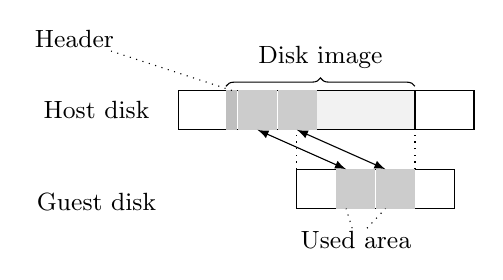
\begin{tikzpicture}[>=latex, font=\small, scale=0.5]
    \path (0,0.5) coordinate (a1);
    \draw (0,0) rectangle (7.5,1);
    \node[left = 0.25cm of a1] (host-disk) {Host disk};

    \draw (3,-2) rectangle (7,-1);
    \node[below = 0.7cm of host-disk] {Guest disk};

    \draw[fill=black!5] (3,0) rectangle (6,1);
    \draw[dotted] (3,-1) -- (3,0);
    \draw[dotted] (6,-1) -- (6,0);

    \path[thick, fill=black!25] (1.2,0) rectangle (1.49,1);
    \path[fill=black!20] (1.51,0) rectangle (2.49,1);
    \path[fill=black!20] (2.51,0) rectangle (3.5,1);

    \path[fill=black!20] (4.,-2) rectangle (4.99,-1);
    \path[fill=black!20] (5.01,-2) rectangle (6,-1);

    \draw[<->] (4.25,-1) -- (2,0);
    \draw[<->] (5.25,-1) -- (3,0);

    \path (4.5,-2) coordinate (a2);
    \node[below =0.25cm of a2, inner sep=1pt] (used) {Used area};

    \draw[dotted] (used) -- (4.25,-2);
    \draw[dotted] (used) -- (5.25,-2);

    \draw[decorate, decoration={brace, amplitude=3pt}, yshift=3pt] (1.2,1) -- (6,1) coordinate[midway] (a3);
    \path (1.35,1) coordinate (a4);
    \node[above = 0.1cm of a3] {Disk image};
    \node[above = 0.5cm of a4, xshift=-2cm, inner sep=1pt] (header) {Header};
    \draw[dotted] (a4) -- (header);
  \end{tikzpicture}
\end{frame}

% \begin{frame}[allowframebreaks]{Последовательный порт}

% \begin{itemize}
% \item Простое устройство
% \item Модель добавляется одной из первых
% \item Поддерживается всеми ОС
% \item Малая скорость (до 115 кбит/с)
% \item Имеет современные реинкарнации (HSUART, SOL)
% \end{itemize}

% Со стороны реальной системы может быть присоединён к
% \begin{itemize}
% \item Реальному COM порту
% \item Виртуальному COM порту
% \item Именованному каналу (pipe)
% \item Сетевому сокету
% \item Эмуляторы терминала
% \item Файлу
% \end{itemize}

% \end{frame}

\section{<<Magic>> Instructions}

\begin{frame}{<<Magic>> Instructions}
  <<Magic>> instruction is a guest processor instruction with simulation
  specific side-effects:
  \begin{itemize}
    \item Stop simulation;
    \item Call to a handler with access to state of the simulated system;
    \item Possible change state;
    \item Resume simulation;
  \end{itemize}
  \vfill
  All the side-effects caused by the <<magic>> instruction are <<immediate>>
  to the VM.
\end{frame}

\begin{frame}{<<Magic>> Instruction Requirements}
  <<Magic>> instruction should not be used in <<regular>> code:
  \begin{itemize}
    \item Non-privileged instruction;
    \item Instruction with not effects outside simulation is the best.
    \item Should be supported by all simulation modes.
  \end{itemize}
\end{frame}

\begin{frame}{<<Magic>> Instruction Candidates}
  \begin{itemize}
    \item \texttt{NOP}\pause --- used a lot by real software.
    \item Intel\reg~IA-32: \texttt{NOP} with prefixes, long \texttt{NOP}.
    \item \texttt{XCHG EAX, EAX} --- used in Bochs as <<magic>> breakpoint.
    \item \texttt{CPUID} --- used in Simics for Intel\reg~IA-32. Cases VM-exit
      in VMX non-root mode.
  \end{itemize}
\end{frame}

\begin{frame}{<<Magic>> Instruction Usage}
  \begin{itemize}
    \item Instrumentation for guest applications.
    \item Data transfer between guest and host --- one word at a time.
    \item Control for remote procedure call (RPC) mechanism.
  \end{itemize}
\end{frame}

\begin{frame}{Special Instructions for Guest to Host Interactions}
  Privileged instructions for implicit guest to host interaction:

  \begin{itemize}
    \item Hypercall --- similar to \texttt{SYSCALL}. \texttt{VMCALL}
      instruction in Intel\reg~IA-32.
    \item Cooperation for virtual memory management --- \texttt{VMFUNC} and
      \texttt{\#VE} in Intel\reg~IA-32.
  \end{itemize}

  Goal --- reduce overhead for most common operations.
\end{frame}

\section{Paravirtual Devices}

\begin{frame}{Paravirtualized Devices}
  \begin{itemize}
    \item More data can be transferred at once.
    \item{<<Real>> device in model's memory map.}
    \item Guest OS needs to be modified: device drivers.
    \item Typical candidates --- high-throughput devices: disks, network cards.
    \item Example: VirtIO.
  \end{itemize}
\end{frame}

\begin{frame}{Paravirtualized Services}
  Interaction with guest OS services:
  \begin{itemize}
    \item Power management,
    \item File system management,
    \item Physical memory usage,
    \item Terminal access,
    \item Time synchronization,
    \item \dots
  \end{itemize}
\end{frame}

\begin{frame}{Paravirtualized Service --- Examples}
  \begin{itemize}
    \item Simics Agent/Matic,
    \item Simics hostfs,
    \item Oracle Virtualbox Guest Additions,
    \item VMware ESX Tools,
    \item Microsoft Hyper-V Integration Services.
  \end{itemize}
\end{frame}

\section{Device Pass-Through}

\begin{frame}{Device Pass-Through}
  A host device can be passed-through for exclusive use by a guest:
  \begin{itemize}
    \item Graphical cards,
    \item Network cards,
    \item Other devices (PCIe/USB).
  \end{itemize}
\end{frame}

\begin{frame}{Device Pass-Through --- Problems}
  \begin{itemize}
    \item Device register access.
    \item Device memory access (DMA).
    \item Interrupt delivery.
  \end{itemize}
  \pause
  \vfill
  More problems:
  \begin{itemize}
    \item Disconnecting device from the host system.
    \item State saving and restoring.
    \item Migration.
  \end{itemize}
\end{frame}

\begin{frame}{Device Pass-Through --- Hardware Support}
  \begin{itemize}
    \item Hardware support (I/O memory management unit).
    \item Examples: Intel VT-d, AMD IOMMU, IBM Translation Control Entry,
      Sun DVMA.
  \end{itemize}
\end{frame}

\section{Networking}

\begin{frame}{Networking}
  \begin{itemize}
    \item Originally created to connected systems of different nature.
    \item Hardware agnostic.
    \item It's possible to choose level of abstraction for guest to host
      border.
  \end{itemize}
\end{frame}

\begin{frame}{OSI/ISO Model}
  \begin{itemize}
    \item Application layer --- service points inside simulation. Respond to a
      specific application protocol: NFS, FTP, Samba, DHCP, \dots
    \item Presentation layer.
    \item Session layer.
    \item Transport layer --- Network Address Translation (NAT). Packets are
      re-translated by host.
    \item Network layer --- Host TUN-driver. IP tunneling.
    \item Data link layer --- Host TAP-driver. Pseudo Ethernet device.
    \item Physical layer --- network card model inside the simulated system.
  \end{itemize}
\end{frame}

\section*{Conclusions}

\begin{frame}{Conclusions}
  \begin{itemize}
    \item Isolation + equivalence $\neq$ efficiency.
    \item Sometimes it is useful to break isolation to get better performance
      and improve user experience --- paravirtualization:
    \begin{itemize}
      \item{<<Magic>> instructions,}
      \item Paravirtualized devices,
      \item Pass-through,
      \item Networking.
    \end{itemize}
  \end{itemize}
\end{frame}

\begin{frame}[allowframebreaks]{Bibliography}
  \begin{thebibliography}{99}
    \bibitem{} Microsoft, ``Hypervisor Top Level Functional Specification''.
    \bibitem{} Microsoft, ``Integration Services'',
      \url{https://technet.microsoft.com/en-us/library/dn798297.aspx}.
    \bibitem{} \texttt{M.~Krasnyansky}, ``Universal TUN/TAP device driver.'',
      \url{http://www.kernel.org/pub/linux/kernel/people/marcelo/linux-2.4/Documentation/networking/tuntap.txt}.
    \bibitem{} Xen Pass-Through, \url{http://wiki.xen.org/wiki/Xen_PCI_Passthrough},
      \url{http://wiki.xen.org/wiki/XenVGAPassthrough},
      \url{http://wiki.xen.org/wiki/XenUSBPassthrough}.
    \bibitem{} Linux paravirt\_ops: \url{http://lwn.net/Articles/194339/},
      \url{http://lwn.net/Articles/225881/}.
    \bibitem{} IBM, ``Virtio: An I/O virtualization framework for Linux'',
      \url{https://developer.ibm.com/articles/l-virtio/}.
  \end{thebibliography}
\end{frame}

\begin{frame}{On the Next Lecture:}
  Programming languages for model development.
\end{frame}

\finalslide

\end{document}
